\documentclass{beamer}
\usepackage{tikz}
\usepackage{pgfplots}
\usepackage{graphicx}
\usepackage{tabu}
\usepackage{booktabs}
\usepackage{fontawesome}
\usetikzlibrary{positioning}
\usetikzlibrary{calc}
%\usetikzlibrary{arrows}

\usefonttheme{professionalfonts}
\usetheme{Boadilla}
\setbeamertemplate{navigation symbols}{}%remove navigation symbols
\hypersetup{pdfstartview={Fit}} % fits the presentation to the window when first displayed
\graphicspath{{./figures/}{./figures/generated/}{./figures/static/}}
\definecolor{gold}{rgb}{1,.776,.153}
\definecolor{maroon}{rgb}{.549,.114,.251}

%Edwards PB, Wanjura WJ, Brown WV: Selective herbivory by Christmas beetles in response to intraspecific variation in Eucalyptus terpenoids. Oecologia 1993, 95:551–557

%Info
\title[Sensitive Genotyping]{Methods for sensitive genotyping in nonmodel organisms}
\titlegraphic{
	\includegraphics[width=.3\linewidth]{gatk_tree_rightwards.pdf}
	\includegraphics[width=.3\textwidth, angle=90]{labeled_tree.jpg}
	}
\date{12/1/19}
\author{Adam Orr\hskip 1em \faicon{twitter}@AdamJOrr}

\begin{document}
\frame{\titlepage}

\begin{frame}{Why are somatic mutations difficult to detect?}

\begin{block}{Mutations are very rare, but sequencing errors are very common.}
\textbf{Sequencing error} alone is \textbf{$\sim10^{-2}$} while mutation rate after error-checking is \textbf{$\sim10^{-9}$}
\end{block}

\begin{itemize}
\item Errors accumulate during PCR prior to sequencing - then propagate.
\item \textit{Taq} $\sim10^{-4}$
\item Technical error from sequencer
\end{itemize}

\includegraphics[trim={1cm 4cm 0 0},clip,width=\linewidth]{pcr_errors.png}

\footnotetext{\tiny{Potapov V, Ong JL (2017) Examining Sources of Error in PCR by Single-Molecule Sequencing}}
\end{frame}

\begin{frame}{Plants Grow Directionally}
\begin{columns}
	\column{.6\linewidth}
		\includegraphics[trim={12cm 2cm 0 22cm},clip,width=\linewidth]{stemcells.jpg}
	\column{.4\linewidth}
		\begin{itemize}
			\item The genetic structure of the plant \textit{should} mirror its physical structure.
		\end{itemize}
\end{columns}
\footnotetext{Heidstra \& Sabatini (2014) Plant and animal stem cells: similar yet different. doi:10.1038/nrm3790}
\end{frame}

\begin{frame}{A Genetic Mosaic}
	\begin{center}
	\includegraphics[width=.6\linewidth]{unlabeled_tree.jpg}
	\end{center}
	\begin{itemize}
		\item Edwards identified as mosaic in 1993\footnote{\textit{Edwards PB, Wanjura WJ, Brown WV. Oecologia 1993, 95:551–557.}}
		\item Sheep pen in Yeoval, New South Wales
		\item Differential oil production gives protection from Christmas beetles
		% \item Is this mutation a controlled process?
	\end{itemize}
\end{frame}

\begin{frame}{Study Methodology}
\begin{columns}

\column{.5\linewidth}
\begin{itemize}
\item Sequence 8 samples in triplicate
\item $\sim$10X coverage for each replicate
\item Align sequence to genome of \textit{Eucalyptus grandis}
\item Use replicates to remove false positives
\end{itemize}

\column{.5\linewidth}
\begin{center}
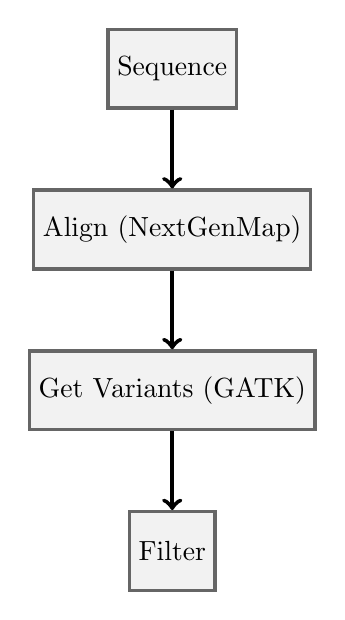
\begin{tikzpicture}[sqnode/.style={rectangle, draw=black!60, fill=black!5,very thick,minimum size=1cm}]
	\node[sqnode] (sequencing) {Sequence};
	\node[sqnode] (alignment) [below = of sequencing] {Align (NextGenMap)};
	\node[sqnode] (varcall) [below = of alignment] {Get Variants (GATK)};
	\node[sqnode] (flt) [below = of varcall] {Filter};
	\draw[ultra thick,->] (sequencing.south) -- (alignment.north);
	\draw[ultra thick,->] (alignment.south) -- (varcall.north);
	\draw[ultra thick,->] (varcall.south) -- (flt.north);
\end{tikzpicture}
\end{center}
\end{columns}
\end{frame}

\begin{frame}{Mutation Pattern Approximately Matches Tree Structure}
\begin{columns}
\column{.5\linewidth}
	\begin{center}
	GATK Best Practices Tree
	\end{center}
	\includegraphics[width=\linewidth]{gatk_tree_rightwards.pdf}
\column{.5\linewidth}
	\begin{center}
	True Tree
	\end{center}
	\includegraphics[width=\linewidth,angle=90]{true_tree.pdf}
\end{columns}
\end{frame}

\begin{frame}{Most Reads Are Not Mapped to the \textit{E. grandis} Reference}
\begin{center}
\includegraphics[width=\linewidth]{bowtie1_hist.pdf}
\end{center}
\end{frame}

\begin{frame}{Approximating a Genome}

Use \textit{E. melliodora} genome as a starting place, then generate a new reference and map to that reference.

\begin{center}
	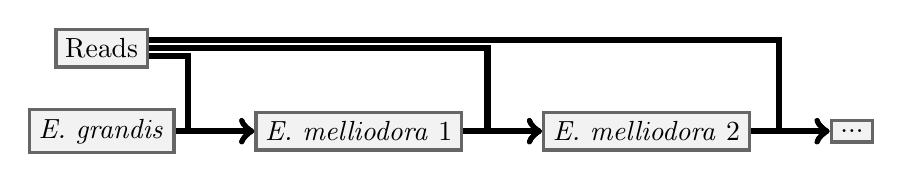
\begin{tikzpicture}[cnode/.style={rectangle,draw=black!60,fill=black!5,very thick}, node distance = 1 cm]
		\node[cnode] (reads){Reads};
		\node[cnode] (eg)[below = .5cm of reads]{\textit{E. grandis}};
		\node[cnode] (em1)[right = of eg]{\textit{E. melliodora} 1};
		\node[cnode] (em2)[right = of em1]{\textit{E. melliodora} 2};
		\node[cnode] (etc)[right = of em2] {...};
		\draw[line width=.8mm,->] ($(reads.east)-(0cm,.1cm)$) -- ($(reads.east)+(.5cm,-.1cm)$) |- (em1.west);
		\draw[line width=.8mm,->] (reads.east) -- ($(reads.east)+(4.3cm,0cm)$) |- (em2.west);
		\draw[line width=.8mm,->] ($(reads.east)+(0cm,.1cm)$) -- ($(reads.east)+(8cm,.1cm)$) |- (etc.west);
		\draw[line width=.8mm,->] (eg) -- (em1);
		\draw[line width=.8mm,->] (em1) -- (em2);
		\draw[line width=.8mm,->] (em2) -- (etc);
	\end{tikzpicture}
\end{center}


\end{frame}

\begin{frame}{Our New Reference Has Fewer Unmapped Reads}
\begin{center}
\includegraphics[width=.95\linewidth]{unmapped_reads.pdf}
\end{center}
\end{frame}

\begin{frame}{Filtering Variants}
\begin{columns}
\column{.5\linewidth}
Remove variants likely from alignment errors:
\begin{itemize}
	\item at sites with excessive depth ($>$500).
	\item with excessive levels of heterozygosity.
	\item within 50 bases of an indel.
	\item in repeat regions 
\end{itemize}
\column{.5\linewidth}
\includegraphics[width=\linewidth]{coverage.png}
\end{columns}
\end{frame}


\begin{frame}{ Filtering and Reference Refinement Improve Tree Topology}
	\begin{columns}
	\column{.5\linewidth}
		\begin{center}
		Predicted Variants
		\end{center}
		\includegraphics[width=\linewidth]{gatk_repeats_removed.pdf}
	\column{.5\linewidth}
		\begin{center}
		True Tree
		\end{center}
		\includegraphics[width=\linewidth,angle=90]{true_tree.pdf}
	\end{columns}
\end{frame}

\begin{frame}{Using Tree Topology Gives Higher Recall Rate}
	\begin{itemize}
	\item Thus, it's reasonable to assume the physical topology when inferring mutations
	\item \textit{DeNovoGear} is a variant-calling method that uses information in the tree topology to call variants.
	\item By simulation, we introduced 14000 mutations on the tree
	\end{itemize}
	\begin{center}
	\begin{tabular}{ c | c }
	\textit{GATK} & \textit{DeNovoGear} \\
	\hline
	3859 mutations & 4193 mutations \\
	27\% & 30\%
	\end{tabular}
	\end{center}
\end{frame}

% \begin{frame}{Randomizing Trees to Estimate False Positive Rate}
% 	\begin{itemize}
% 		\item Does using a phylogeny increase our false positive rate?
% 		\item Simulate 100 trees maximally distant from the true tree.
% 		\item Does our pipeline detect variation where there shouldn't be any?
% 		\item \textbf{All} sites detected were variable sites.
% 	\end{itemize}
% \end{frame}

\begin{frame}{Mutation Rates}
\begin{columns}
\column{.5\linewidth}
\begin{itemize}
\item Detected $90$ mutations.
\item $20$ mutations in genes.
\item Estimated recall of $\sim30\%$.
\item $90\times\frac{1}{.3}=300$ mutations.
\item $\sim3.3$ mutations per meter of length
\item $2.7\times10^{-9}$ mutations per base per meter
\item Somatic mutations account for $\sim55$ mutations per leaf tip.
\end{itemize}
\column{.5\linewidth}
\includegraphics[width=\linewidth]{labeled_nodes_tree.jpg}
\end{columns}
\end{frame}

\begin{frame}{Model Parameters}
\begin{columns}
\column{.5\linewidth}
We studied \textit{one} individual, but we can make conjectures about the population.
\begin{itemize}
\item The average height of a eucalypt is $22.5$ M
\item Mutation rate per base, per generation is $6.2\times10^{-8}$
\item We estimated $\theta = 0.025$
\item Since $\theta = 4N_{e}\mu$, $N_{e} = 102,000$
\end{itemize}
\column{.5\linewidth}
\includegraphics[width=\linewidth]{labeled_nodes_tree.jpg}
\\
\end{columns}

\vskip 1em

\hrule

\vskip 1em

This per-generation rate is $\sim10\times$ larger than \textit{Arabidopsis}, but \textit{Eucalyptus} is $100\times$ larger.

\end{frame}

\begin{frame}{Chapter 3 - Base Quality Score Recalibration in Non-model Organisms}

Errors make variant calling difficult - but we can predict them.

\begin{columns}
	\column{.5\linewidth}
	\begin{itemize}
		\item FASTQ format data has a quality score
		\item Quality scores represent $P(error)$ on a phred scale.
		\begin{displaymath}
		P(error) = 10^{\frac{-Q}{10}}
		\end{displaymath}
		\begin{displaymath}
		Q = -10\log_{10}{P(error)}
		\end{displaymath}
	\end{itemize}
	\column{.5\linewidth}
	\begin{tabular}{l r} \toprule
	\bfseries Quality Score & \bfseries $P(error)$ \\
	\hline
	1 & 0.8 \\
	2 & 0.6 \\
	3 & 0.5 \\
	4 & 0.4 \\
	5 & 0.3 \\
	6 & 0.3 \\
	7 & 0.2 \\
	8 & 0.2 \\
	9 & 0.1 \\
	\bfseries 10 & \bfseries  0.1 \\
	\bfseries 20 & \bfseries 0.01 \\
	\bfseries 30 & \bfseries 0.001 \\
	\bfseries 40 & \bfseries 0.0001 \\
	\end{tabular}
\end{columns}

\end{frame}

\begin{frame}{Quality scores are predictions}
\begin{columns}
\column{.5\linewidth}
\begin{itemize}
\item A quality score is a \textbf{prediction} about whether a base call is correct.
\item Predictions are said to be \textbf{calibrated} if the predicted event occurs as often as predicted.
\item The weather forecast contains a \textbf{prediction} about whether it will rain.
\item If it rains on a day with a 30\% chance of rain, what does that mean?
\end{itemize}
\column{.5\linewidth}
\begin{tikzpicture}
\begin{axis}[width = .9\textwidth, xlabel={Predicted Probability}, ylabel={Measured Frequency}]
\addplot[black,samples = 50,domain=0:1]{x};
\end{axis}
\end{tikzpicture}
\end{columns}
\end{frame}

\begin{frame}{Quality scores aren't well-calibrated}
\begin{columns}
\column{.5\linewidth}
\begin{itemize}
\item If quality scores \textit{were} well-calibrated, it would be easier to identify errors
\item Base Quality Score Recalibration can be done to fix calibration issues.
\item Current GATK method for BQSR require a database of variable sites in your data
then assumes mismatches at nonvariable sites are errors.
\end{itemize}
\column{.5\linewidth}
\includegraphics[width=.95\linewidth]{raw_gatk.pdf}
\end{columns}
\end{frame}

\begin{frame}{BQSR uses a linear model to determine how much to adjust each quality score}
\centering
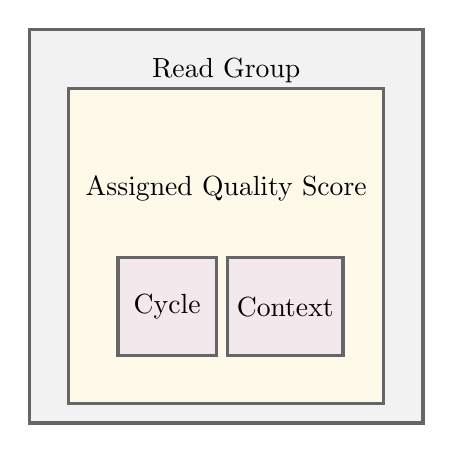
\begin{tikzpicture}[align=center, sqnode/.style={rectangle,draw=black!60,fill=black!5,very thick,minimum size=1cm}, node distance = 1 cm]
	\node[sqnode,align=center,above,minimum size=5cm](rg) at (2,0){};
	% \draw[help lines] (0,0) grid (16,16);
	\node[](rglab) at (2,4.5){Read Group};
	\node[sqnode, align=center,above,minimum size=4cm,fill=gold!10](q) at (2,.25){};
	\node[](qlab) at (2,3){Assigned Quality Score};
	\node[sqnode, minimum size = 1.25 cm,fill=maroon!10] at (1.25,1.5) {Cycle};
	\node[sqnode, minimum size = 1.25 cm,fill=maroon!10] at (2.75,1.5) {Context};
\end{tikzpicture}
\end{frame}

\begin{frame}{Questions}
\begin{itemize}
	\item How effective is BQSR, particularly if the reference and database of known variation are not good?
	\item What is the impact of BQSR on downstream variant calls? 
\end{itemize}
\end{frame}

\begin{frame}{BQSR is vulnerable to false negatives in the database of variable sites}
\begin{columns}
\column{.5\linewidth}
\includegraphics[width=.95\linewidth]{fpr.pdf}
\column{.5\linewidth}
\includegraphics[width=.95\linewidth]{fnr.pdf}
\end{columns}
\end{frame}

\begin{frame}{Alternative approaches get around using a database of variable sites}
\begin{itemize}
	\item Lacer uses singular value decomposition
	\item ReQON limits the number of errors there can be at a site
	\item Syntheic spike-ins
\end{itemize}
\end{frame}

\begin{frame}{Error correctors can find some errors without a reference}
\begin{columns}
\column{.5\linewidth}
\begin{itemize}
\item Error correction methods exist that use k-mers to identify errors rather than an alignment and reference.
\item Most error correctors don't update quality scores.
\end{itemize}

\column{.5\linewidth}
\includegraphics[width=.95\linewidth]{raw_lighter.pdf}
\end{columns}
\end{frame}

\begin{frame}{K-mer-Based Base Quality score recalibration}
\begin{columns}
\column{.5\linewidth}
\begin{itemize}
\item Combining error correction and BQSR is effective
\item Method implemented in \texttt{kbbq} software
\end{itemize}
\column{.5\linewidth}
\includegraphics[width=.95\linewidth]{comparison.pdf}
\end{columns}
\end{frame}

\begin{frame}{Future Plans}
Evaluate downstream impact on quality of variant calls
\begin{itemize}
\item F-score of returned calls
\item Statistics of GATK and other callers influenced by quality scores.
\item Run \texttt{kbbq} on the Eucalyptus data and find how that changes the distribution of quality scores and the number of detected variants.
\end{itemize}
\end{frame}

\begin{frame}{Chapter 4 - Base Quality Score Recalibration in Long Reads}
\begin{itemize}
\item PacBio hi-fi reads are a consensus of many sub-reads; do these consensus reads have meaningful quality scores?
\item Nanopore reads are said to be well-calibrated, but in Illumina different runs can produce different error profiles; is this the same in Nanopore?
\item Genome In A Bottle has Illumina, PacBio, and Nanopore sequencing of the same sample.
\end{itemize}
\end{frame}

\begin{frame}{Methods}
\item Check data for calibration; if it's not well calibrated, try using GATK/\texttt{kbbq} and see if it works.
\item Nanopore uses 5 or 6bp basecalling models, so the context covariate in this case should be that long.
\item Does logistic regression make more sense for this data?
\end{frame}


\begin{frame}{Acknowledgements}
\begin{itemize}
\item Advisor: Reed Cartwright\hskip 1em \faicon{twitter}@MinionLab
\item Robert Lanfear, Australian National University\hskip 1em \faicon{twitter}@RobLanfear
\end{itemize}

Pipeline: \faicon{github} \url{https://github.com/adamjorr/somatic-variation}

KBBQ: \faicon{github} \url{https://github.com/adamjorr/kbbq}

Talk: \faicon{github} \url{https://github.com/adamjorr/talks}

\vfill

\begin{columns}
\column{.4\linewidth}
	\includegraphics[width=.9\linewidth]{lab_logo.pdf}
	\\~\\
	\includegraphics[width=.9\linewidth]{biodesign_logo.pdf}
\column{.4\linewidth}
	\includegraphics[width=.9\linewidth]{sols_logo.pdf}
	\\~\\
	This work is supported by grants NIH R01-HG007178 and NSF DBI-1356548.
\end{columns}

\end{frame}

\end{document}
